\documentclass[15pt]{article}

% Language setting
% Replace `english' with e.g. `spanish' to change the document language
\usepackage[english]{babel}

% Set page size and margins
% Replace `letterpaper' with `a4paper' for UK/EU standard size
\usepackage[letterpaper,top=2cm,bottom=2cm,left=3cm,right=3cm,marginparwidth=1.75cm]{geometry}

% Useful packages
\usepackage{amsmath}
\usepackage{graphicx}
\usepackage[colorlinks=true, allcolors=blue]{hyperref}
\usepackage{listings}
\usepackage{color}

\definecolor{dkgreen}{rgb}{0,0.6,0}
\definecolor{gray}{rgb}{0.5,0.5,0.5}
\definecolor{mauve}{rgb}{0.58,0,0.82}

\lstset{frame=tb,
  language=Java,
  aboveskip=3mm,
  belowskip=3mm,
  showstringspaces=false,
  columns=flexible,
  basicstyle={\small\ttfamily},
  numbers=none,
  numberstyle=\tiny\color{gray},
  keywordstyle=\color{blue},
  commentstyle=\color{dkgreen},
  stringstyle=\color{mauve},
  breaklines=true,
  breakatwhitespace=true,
  tabsize=3
}

\title{Brownies - Editorial}
\author{Timothy Gao}
\date{}

\begin{document}
\maketitle

First, it helps to reformulate the problem so it's more clear what we're working with and make it easier to approach. Essentially, we are given an $N * M$ grid ($1 \leq N * M \leq 10^6$) of 0s which are fixed and Xs which we can choose the integer value of. We wish to find for each cell in the grid the number of possible values it can take on, such that:

\begin{enumerate}
    \item The value of two neighboring cells differ by at most one.
    \item Every cell is strictly greater than at least one of its adjacent neighbors, unless the cell has a value of 0.
\end{enumerate}

\section{Initial Observations}

Trivially, the number of possible values for each 0 cell is just 1, since its value is fixed.

I claim that if we fix which cells must be 0, the value of the remaining X cells are uniquely determined.

Consider the structure such a grid. The grid is made up of several "islands" of Xs, which are connected components separated by 0s. The cells immediately bordering a 0 is highlighted in yellow in Figure \ref{fig:bordering} below.

\begin{figure}[h]
\centering
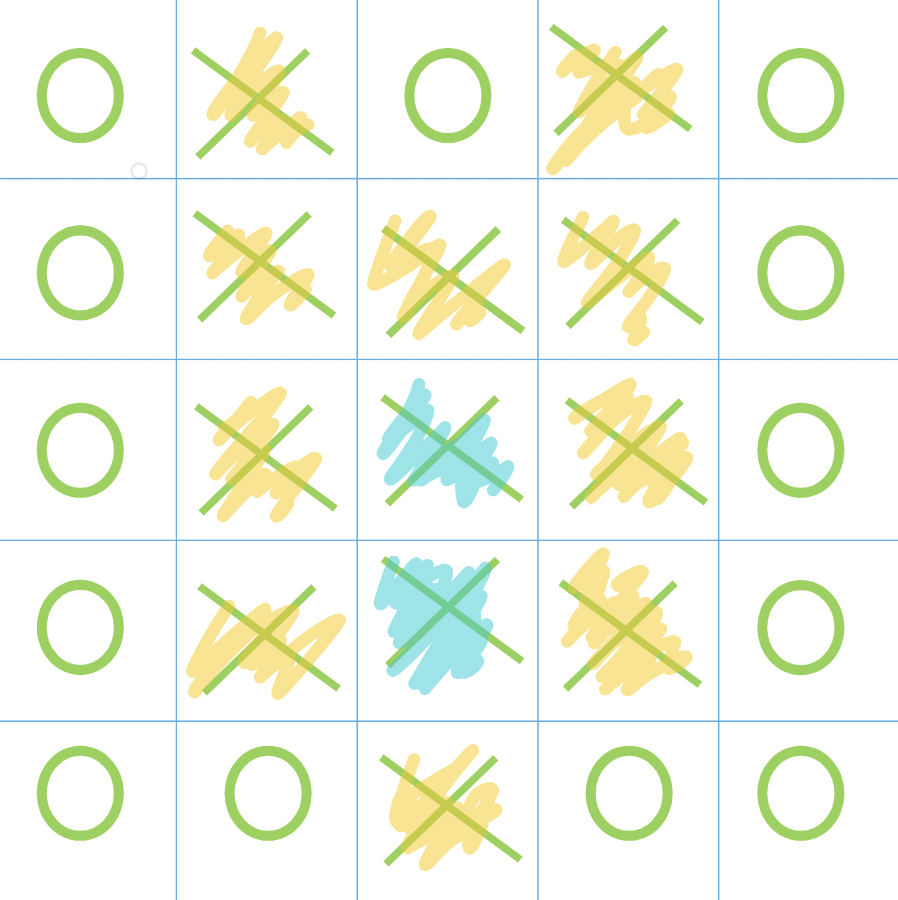
\includegraphics[width=0.3\textwidth]{Grid.png}
\caption{\label{fig:bordering}Example Grid with one island}
\end{figure}

By definition, these cells cannot be 0 because we already fixed which cells are are 0. Therefore, they must be 1 due the first condition. Now, all cells bordering these cells, highlighted in blue, must take on a value of 2. We can prove this by contradiction. Imagine a cell $C_a$ bordering a yellow cell is not 2. Then there must exist another cell $C_b \le C_a-1$ bordering $C_a$ for the second condition be met, which means there exist another cell $C_c \leq C_b-1$, and that cell must have another cell less than it, and so on. As a result, one of the Xs must eventually be reduced to 0, which contradicts our initial condition that we already fixed which cells are 0. We can recursively apply this logic layer after layer (note that in Figure \ref{fig:bordering} we only have two layers, yellow and blue). Each outer layer must all have the same value, which is one greater than the value of the inner layer it surrounds. In general, after we fix which cells must be 0, the values of each remaining X cell is uniquely determined to be its Manhattan Distance ($|x_i - x_j| + |y_i - y_j|$) from the closest 0 cell. More formally, $M = $
$\displaystyle \min_{(x_1, y_1),\dots (x_T, y_T)} |x - x_i| + |y - y_i|$ where $(x_i, y_i)$ are the coordinates of the $i$th 0 cell.

\section{Arriving at the Solution}

As a consequence of our Manhattan Distance argument, to maximize the values of each X cell, we would greedily fix as few 0 cells as possible. This means we only include the initial cells that must be 0, and don't fix any of the X cells to be 0. 

Now, I claim that the value of each X cell in all can be any value in the range $[0, M]$ where M is the maximum value it can attain over all possible valid grids. This can be proven constructively. Considering an X cell $A$, if we fix a different X cell $B$ in the island of $A$ to be 0, then we can move it closer and closer $A$, reducing the Manhattan Distance and value of $A$ by one each step.

Our conclusions above means that the number of possible values would be $M+1$ for each X cell, and $1$ for each 0 cell. To find these values quickly, we perform a multi-source BFS in $O(N*M)$ starting from the 0 cells, which fits comfortably under the time limit.

Finally, one last edge case we have to consider is if all cells are X. In that case, $M$ would be the maximum Manhattan distance from any cell in the grid, but we effectively only have to consider its distance to the four corner cells.

\section{Code}
\begin{lstlisting}
//@timothyg

#include <bits/stdc++.h>
 
using namespace std;
 
typedef long long ll;
typedef pair<int, int> pii;

#define pb push_back

#define f first
#define s second

int rDir[4] = {1, -1, 0, 0}, cDir[4] = {0, 0, 1, -1};

int main(){
    ios_base::sync_with_stdio(false); cin.tie(0);
    
    int N, M, hasZero = 0; cin >> N >> M;
    vector<vector<int>> grid(N, vector<int>(M)), res(N, vector<int>(M));
    queue<array<int, 3>> bfs;
    for(int i = 0; i<N; i++){
        string str; cin >> str;
        for(int j = 0; j<M; j++){
            grid[i][j] = str[j] == 'X';
            if(!grid[i][j]) hasZero = 1, bfs.push({i, j, 1});
        }
    }
    //edge case if every cell is X -- one of the elements must be 0
    if(!hasZero){
        for(int i = 0; i<N; i++){
            for(int j = 0; j<M; j++){
                int farthestRow = max(i, N - 1 - i);
                int farthestCol = max(j, M - 1 - j);
                cout << (farthestRow + farthestCol + 1) << " ";
            }
            cout << '\n';
        }
        return 0;
    }

    while(!bfs.empty()){
        array<int, 3> cur = bfs.front(); bfs.pop();
        if(res[cur[0]][cur[1]] != 0) continue;
        res[cur[0]][cur[1]] = cur[2];
        for(int i = 0; i < 4; i++){
            int dR = cur[0] + rDir[i], dC = cur[1] + cDir[i];
            if(dR >= 0 && dC >= 0 && dR < N && dC < M){
                bfs.push({dR, dC, cur[2] + 1});
            }
        }
    }

    for(int i = 0; i<N; i++){
        for(int j = 0; j<M; j++){
            cout << res[i][j] << " ";
        }
        cout << '\n';
    }

    return 0;
}
\end{lstlisting}

\end{document}